% ==========================================================
\section{PGFPlots (高级绘图)}
% ==========================================================

\subsection{2D Function Plots (二维函数图)}

\subsubsection{功能介绍 (Introduction)} 

PGFPlots 是基于 TikZ 构建的宏包,专门用于绘制科学数据图表。它提供了坐标轴自动缩放、刻度管理等高级功能。

PGFPlots is a package built on top of TikZ, specifically designed for plotting scientific data. It provides advanced features like automatic axis scaling and tick management.

\vspace{0.5em}
\subsubsection{代码展示 (Code)}

\begin{lstlisting}[language=TeX]
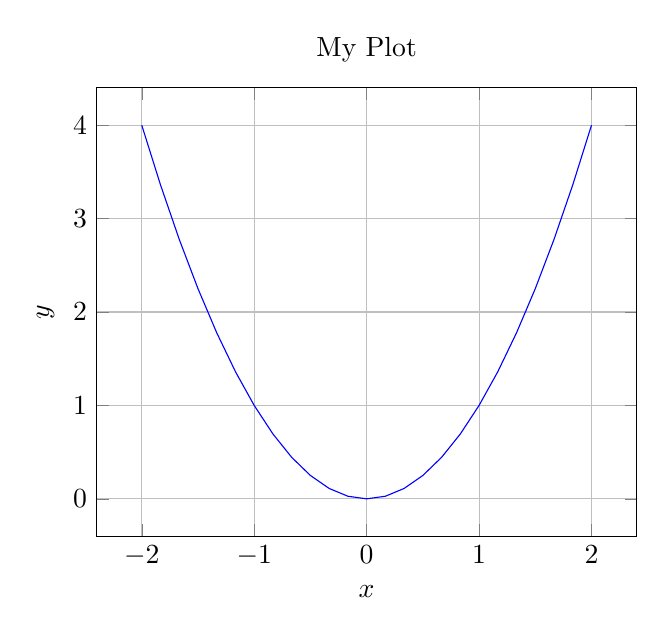
\begin{tikzpicture}
    \begin{axis}[
        title={My Plot},
        xlabel={$x$},
        ylabel={$y$},
        grid=major
    ]
    \addplot[blue, domain=-2:2] {x^2};
    \end{axis}
\end{tikzpicture}
\end{lstlisting}

\subsubsection{语法详解 (Syntax)}

\begin{itemize}
    \item \code{axis}: 坐标轴环境。
    \item \code{\\addplot}: 添加数据系列。
    \item \code{domain}: 定义自变量范围。
\end{itemize}

\subsubsection{效果展示 (Effect)}

\begin{center}
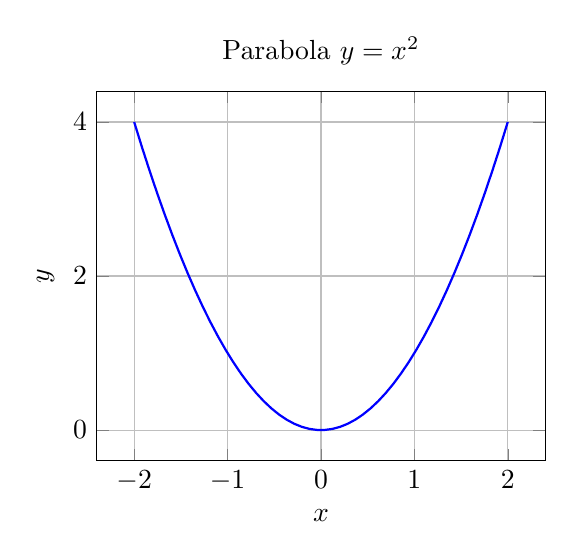
\begin{tikzpicture}
    \begin{axis}[
        width=0.6\textwidth,
        title={Parabola $y=x^2$},
        xlabel={$x$},
        ylabel={$y$},
        grid=major
    ]
    \addplot[blue, thick, domain=-2:2, samples=50] {x^2};
    \end{axis}
\end{tikzpicture}
\end{center}

\subsection{3D Surface Plots (三维曲面图)}

\subsubsection{功能介绍 (Introduction)} 

PGFPlots 还可以绘制令人印象深刻的三维曲面图。

PGFPlots can also draw impressive 3D surface plots.

\vspace{0.5em}
\subsubsection{代码展示 (Code)}

\begin{lstlisting}[language=TeX]
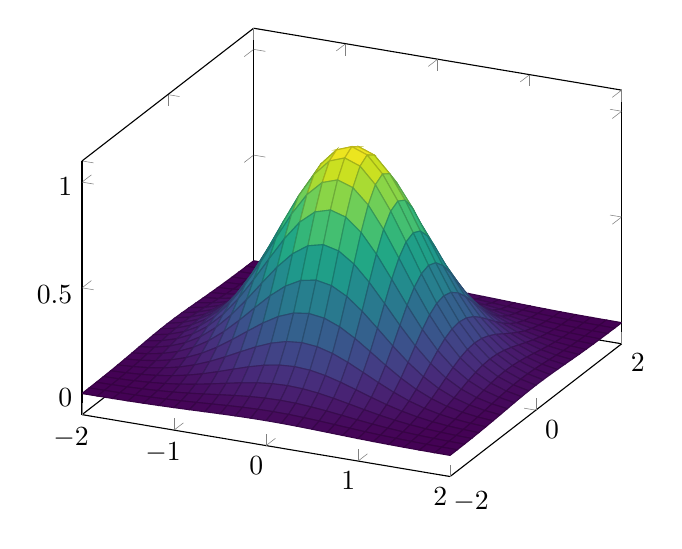
\begin{tikzpicture}
    \begin{axis}[colormap/viridis]
    \addplot3[surf, domain=-2:2] {exp(-x^2-y^2)};
    \end{axis}
\end{tikzpicture}
\end{lstlisting}

\subsubsection{语法详解 (Syntax)}

\begin{itemize}
    \item \code{\\addplot3[surf]}: 绘制三维曲面。
    \item \code{colormap/viridis}: 设置配色方案。
\end{itemize}

\subsubsection{效果展示 (Effect)}

\begin{center}
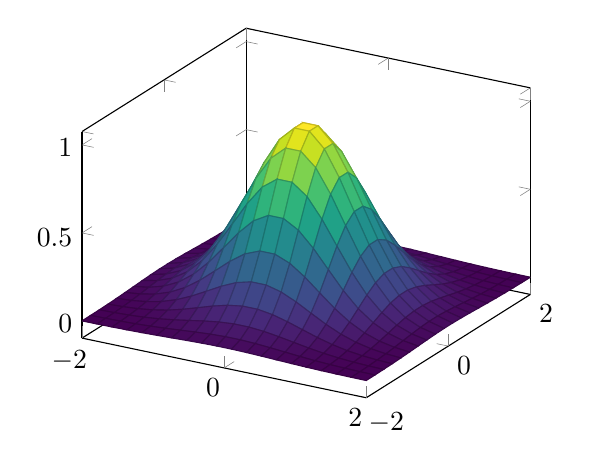
\begin{tikzpicture}
    \begin{axis}[
        width=0.6\textwidth,
        colormap/viridis,
        view={30}{30}
    ]
    \addplot3[surf, domain=-2:2, samples=20] {exp(-x^2-y^2)};
    \end{axis}
\end{tikzpicture}
\end{center}
